%% Chapter 1 — Axiomatic Basis and S-Entropy Calculus
%%
%% Source material:
%%   docs/sources/unconstrained-subtask-recursion.tex  (primary)
%%   README.md §2
%%
%% This chapter states the two axioms, derives the S-functional and
%% all its structural properties, proves the Triple Equivalence via
%% explicit functors, and establishes the Unconstrained Subtask Theorem
%% and Circular Validation.  Everything downstream builds on this chapter
%% without re-deriving.

\chapter{Axiomatic Basis and S-Entropy Calculus}
\label{ch:axioms}

\section{The Two Axioms}
\label{sec:axioms}

The entire framework rests on two axioms whose joint content is that every
physical observer is a \emph{finite} entity interacting with a \emph{finite}
world.  No other metaphysical machinery is required.

\begin{axiom}[Bounded Phase Space]
\label{ax:bounded-phase}
Every physical system with finite energy $E$ and spatial extent $R$ possesses a
phase space $\Omega$ of finite Liouville measure:
\[
  \mu(\Omega) < \infty .
\]
\end{axiom}

\begin{axiom}[Categorical Observation]
\label{ax:categorical-obs}
Any observer $\mathcal{R}$ with finite resolution $\varepsilon > 0$ partitions
$\Omega$ into a finite collection of cells:
\[
  \Pi(\Omega) = \bigl\{ C_1, C_2, \ldots, C_N \bigr\}, \qquad
  N = |\Pi(\Omega)| < \infty .
\]
The cells are pairwise disjoint and their union covers $\Omega$:
$C_i \cap C_j = \emptyset$ for $i \neq j$ and $\bigcup_i C_i = \Omega$.
\end{axiom}

\begin{remark}
\Cref{ax:bounded-phase} is the standard assumption of classical and quantum
statistical mechanics: the partition function converges.  \Cref{ax:categorical-obs}
is the operational statement that any measurement apparatus has a minimal
distinguishable volume $\delta^d > 0$, where $d$ is the dimension of the
phase space.  The two axioms together imply all results of this monograph
without further assumptions.
\end{remark}

\begin{theorem}[Forced Partitioning]
\label{thm:forced-partitioning}
Let $\mathcal{R}$ be an observer with minimal distinguishable phase-space volume
$\delta^d > 0$.  Then the number of cells in any partition compatible with
$\mathcal{R}$ satisfies
\[
  N \;\leq\; \left\lfloor \frac{\mu(\Omega)}{\delta^d} \right\rfloor
  \;<\; \infty .
\]
In particular, the observer cannot resolve individual points of $\Omega$.
\end{theorem}

\begin{proof}
By \Cref{ax:bounded-phase}, $\mu(\Omega) < \infty$.  By
\Cref{ax:categorical-obs}, each cell $C_i$ satisfies $\mu(C_i) \geq \delta^d$
because $\mathcal{R}$ cannot distinguish states separated by less than $\delta^d$
in Liouville measure.  Disjointness of the cells gives
\[
  \mu(\Omega) = \sum_{i=1}^{N} \mu(C_i) \;\geq\; N \cdot \delta^d ,
\]
which rearranges to $N \leq \mu(\Omega)/\delta^d$.  Since the right-hand side
is finite, $N < \infty$.  A single point has Liouville measure zero, so no
collection of finitely many cells of positive measure can resolve individual
points.
\end{proof}

\begin{corollary}[Point-Resolution Impossibility]
\label{cor:point-resolution}
Under \Cref{ax:bounded-phase,ax:categorical-obs}, no bounded observer can
determine the exact state $x \in \Omega$; it can only determine the cell
$C_i \ni x$.
\end{corollary}

These results immediately imply that all information about a system available
to any bounded observer is \emph{cell-level} information.  The consequences for
biology, medicine, and disease are explored throughout the monograph.

\section{Partition Geometry}
\label{sec:partition-geometry}

The structure of an observer's partition is not arbitrary.  Physical symmetry
and hierarchical organisation constrain the allowable partition coordinates.

\begin{definition}[Partition Coordinates]
\label{def:partition-coords}
A partition cell is labelled by the quadruple $(n, \ell, m, s)$ where:
\begin{enumerate}[(i)]
  \item $n \geq 1$ is the \emph{nesting depth} — the number of hierarchical
    levels in the partition;
  \item $\ell \in \{0, 1, \ldots, n-1\}$ is the \emph{partition complexity}
    index at the current level;
  \item $m \in \{-\ell, -\ell+1, \ldots, \ell\}$ is the \emph{orientation}
    index of the cell within level $\ell$;
  \item $s \in \{-\tfrac{1}{2}, +\tfrac{1}{2}\}$ is the \emph{chirality}
    selector distinguishing two otherwise equivalent sub-cells.
\end{enumerate}
\end{definition}

\begin{proposition}[Capacity Formula]
\label{prop:capacity}
The total number of cells at nesting depth $n$ is
\[
  \Capacity(n) \;=\; 2n^2 .
\]
\end{proposition}

\begin{proof}
For fixed $n$, the index $\ell$ ranges over $\{0, \ldots, n-1\}$.  For each
$\ell$, the orientation index $m$ takes $2\ell + 1$ values.  The chirality
selector $s$ doubles each count.  Summing over all levels:
\[
  \Capacity(n) \;=\; 2 \sum_{\ell=0}^{n-1} (2\ell + 1)
  \;=\; 2 \cdot n^2 ,
\]
where the identity $\sum_{\ell=0}^{n-1}(2\ell+1) = n^2$ is the standard sum
of the first $n$ odd integers.
\end{proof}

\begin{remark}
The formula $\Capacity(n) = 2n^2$ reproduces the atomic shell capacity of
quantum mechanics (2, 8, 18, 32, \ldots for $n = 1, 2, 3, 4, \ldots$).  This
is not a coincidence: both arise from the same angular-momentum bookkeeping
applied to a hierarchy of distinguishable states.  The partition framework thus
provides a combinatorial derivation of the Pauli capacity of quantum shells
from purely observational axioms.
\end{remark}

\begin{definition}[Partition Depth]
\label{def:partition-depth}
The \emph{partition depth} $\Depth$ of a partition $\Pi$ is the amount of
hierarchical structure needed to uniquely specify a cell within $\Pi$:
\[
  \Depth(\Pi) \;=\; \sum_{i} \log_b k_i ,
\]
where $k_i$ is the branching factor at level $i$ and $b \geq 2$ is the base
of the logarithm.  $\Depth$ is measured in \emph{partition bits} (base-2)
or \emph{partition nats} (base-$e$).
\end{definition}

\begin{theorem}[Depth–Entropy Equivalence]
\label{thm:depth-entropy}
The partition depth $\Depth$ and the Boltzmann entropy $S_P$ of the
associated microstate distribution are related by
\[
  S_P \;=\; \kB \cdot \Depth \cdot \ln b ,
\]
where $\kB$ is Boltzmann's constant and $b$ is the logarithm base.
\end{theorem}

\begin{proof}
The partition places uniform probability $p = 1/b^{\Depth(\Pi)}$ on each
of the $b^{\Depth}$ equiprobable cells (uniform prior by the maximum-entropy
principle under the cell constraint).  The Boltzmann entropy is
\[
  S_P \;=\; -\kB \sum_i p \ln p
  \;=\; -\kB \cdot b^{\Depth} \cdot \frac{1}{b^{\Depth}} \cdot
  \ln \frac{1}{b^{\Depth}}
  \;=\; \kB \cdot \Depth \cdot \ln b .  \qedhere
\]
\end{proof}

\begin{definition}[Partition Time]
\label{def:partition-time}
The \emph{partition time} $\tau_p$ is the minimal time required to carry out
one act of partitioning, set by the time–energy uncertainty relation:
\[
  \tau_p \;=\; \frac{\hbar}{\kB T} \;>\; 0 .
\]
\end{definition}

\begin{theorem}[Residue Principle]
\label{thm:residue}
Because partitioning takes finite time $\tau_p > 0$ and the system continues
to evolve during $\tau_p$, every partition leaves a \emph{residue} — a
non-zero entropy contribution arising from the evolution that occurred while
the partition was being made.  Formally, for any partition $\Pi$ of $\Omega$
performed over interval $[t_0, t_0 + \tau_p]$,
\[
  \Delta S_{\mathrm{res}}(\Pi) \;=\; S_P(\Pi(t_0 + \tau_p)) - S_P(\Pi(t_0))
  \;>\; 0 .
\]
\end{theorem}

\begin{proof}
Let $\Phi_t : \Omega \to \Omega$ be the Hamiltonian flow.  During $[t_0,
t_0 + \tau_p]$, the system moves from $x(t_0)$ to $x(t_0 + \tau_p)$.  The
partition $\Pi$ is constructed with respect to the state at $t_0$, but the
system is measured at $t_0 + \tau_p$.  The mismatch between the partition
and the evolved state contributes
\[
  \Delta S_{\mathrm{res}} \;\geq\; \kB \ln \frac{\mu(\Phi_{\tau_p}(C_i))}{\mu(C_i)}
\]
for the cell $C_i$ containing $x(t_0)$.  By Liouville's theorem, $\Phi_{\tau_p}$
preserves measure, but the image $\Phi_{\tau_p}(C_i)$ generally overlaps
multiple cells of $\Pi$, increasing the conditional entropy.  Since $\tau_p > 0$
and the flow is non-trivial, this overlap is positive, giving
$\Delta S_{\mathrm{res}} > 0$.
\end{proof}

\begin{proposition}[Partition Gradient Flow]
\label{prop:gradient-flow}
In the space of partition configurations, system trajectories satisfy the
gradient flow equation
\[
  \frac{dx}{dt} \;=\; -\gamma \,\nabla \Depth(x) ,
\]
where $\gamma > 0$ is a dissipation coefficient.  Systems therefore evolve
toward configurations of lower partition depth — toward greater simplicity
and coarser self-description.
\end{proposition}

\begin{proof}
The partition depth $\Depth(x)$ plays the role of a Lyapunov functional.
By \Cref{thm:depth-entropy}, $\Depth$ is monotonically related to entropy
production.  Standard arguments from irreversible thermodynamics (the
minimum entropy-production principle for near-equilibrium systems) give the
gradient flow as the steepest-descent dynamics in partition-depth space.
The dissipation coefficient $\gamma = \tau_p^{-1} \cdot \kB T / \mu$ follows
from the fluctuation-dissipation theorem applied to partition fluctuations.
\end{proof}

\section{The S-Functional}
\label{sec:s-functional}

The \emph{S-functional} formalises the epistemic distance between a receiver
and a target cell.  It is the central object of the entire theory.

\begin{definition}[S-Functional]
\label{def:s-functional}
For a receiver $\mathcal{R}$, a system state $x \in \Omega$, and a target cell
$C \subset \Omega$, the \emph{S-functional} is
\[
  S(\mathcal{R},\, x;\, C)
  \;=\;
  \inf_{x' \in \Pi(D(x))} \dcat(x', C) \;+\; \beta ,
\]
where:
\begin{itemize}
  \item $D(x)$ is the resolution cell of $\mathcal{R}$ containing $x$;
  \item $\Pi(D(x))$ is the partition of $D(x)$ induced by $\mathcal{R}$;
  \item $\dcat$ is the categorical distance (\Cref{def:categorical-distance});
  \item $\beta > 0$ is the \emph{irreducible floor} (proved positive in
    \Cref{ch:epistemic}).
\end{itemize}
\end{definition}

\begin{definition}[Categorical Distance]
\label{def:categorical-distance}
The \emph{categorical distance} $\dcat : \Omega \times 2^\Omega \to [0,\infty)$
is defined by
\[
  \dcat(x', C) \;=\; 1 - \mathbf{1}_C(x') ,
\]
where $\mathbf{1}_C$ is the indicator function of $C$.  Equivalently,
$\dcat(x', C) = 0$ if $x' \in C$ and $\dcat(x', C) = 1$ if $x' \notin C$.
\end{definition}

\begin{remark}
The categorical distance is independent of spatial distance and optical
opacity: two states that are categorically proximate (same cell) remain so
regardless of whether they are spatially near or far, visible or occluded.
This is the content of the Opacity Independence corollary
(\Cref{cor:opacity-independence}) proved in \Cref{sec:triple-equivalence}.
\end{remark}

\begin{definition}[S-Entropy Space]
\label{def:s-space}
The \emph{S-entropy space} is the triple
\[
  \Sspace \;=\; \bigl\{ (\Sk, \St, \Se) \bigr\} \;\subset\; [0,1]^3 ,
\]
with \emph{S-coordinate} $\Scoord = (\Sk, \St, \Se)$ and components:
\begin{enumerate}[(i)]
  \item $\Sk$ — \emph{kinematic S-entropy}: uncertainty in the position and
    momentum of the system within its resolution cell;
  \item $\St$ — \emph{thermodynamic S-entropy}: free-energy cost of
    localising the system to the target cell, normalised by $\kB T$;
  \item $\Se$ — \emph{epistemic S-entropy}: information deficit between the
    receiver's representation and the target cell.
\end{enumerate}
\end{definition}

\begin{theorem}[Entropy Identity]
\label{thm:entropy-identity}
The total S-entropy satisfies
\[
  S(\mathcal{R}, x; C)
  \;=\; \kB \cdot \Depth(\Pi) \cdot \ln n ,
\]
where $n$ is the nesting depth of the partition $\Pi$ induced by $\mathcal{R}$
on $D(x)$.  In S-coordinate notation, $\Scoord = (\Sk, \St, \Se)$ with
$\Sk + \St + \Se = \kB \Depth \ln n$.
\end{theorem}

\begin{proof}
By \Cref{def:s-functional}, $S(\mathcal{R}, x; C) = \inf_{x' \in \Pi(D(x))}
\dcat(x', C) + \beta$.  The infimum equals $\beta$ when $C$ intersects the
resolution cell $D(x)$ (so some $x' \in C$ is available) and equals
$1 + \beta$ when $C$ is disjoint from $D(x)$.  For the generic intermediate
case where $C$ partially overlaps $D(x)$, the infimum is the fractional area
measure $1 - \mu(C \cap D(x))/\mu(D(x))$, plus $\beta$.  Expressing
$\mu(D(x))$ in terms of the partition depth via \Cref{def:partition-depth}
and applying \Cref{thm:depth-entropy} with base $b = n$ yields the identity.
The decomposition $\Scoord = (\Sk, \St, \Se)$ follows by projecting the
total onto the three phase-space subspaces (position-momentum, energy, and
information).
\end{proof}

\begin{proposition}[Monotonicity of S-Functional under Refinement]
\label{prop:monotone-refinement}
If $\Pi' \leq \Pi$ (i.e., $\Pi'$ refines $\Pi$), then for all $x$ and $C$,
\[
  S(\mathcal{R}', x; C) \;\leq\; S(\mathcal{R}, x; C) ,
\]
where $\mathcal{R}'$ is the receiver inducing $\Pi'$.  Finer partitions yield
lower (or equal) S-values, bounded below by $\beta$.
\end{proposition}

\begin{proof}
Since $\Pi'$ refines $\Pi$, each cell of $\Pi'$ is contained in a cell of
$\Pi$.  Thus $\Pi'(D'(x)) \subseteq \Pi(D(x))$ and the infimum in
\Cref{def:s-functional} is taken over a smaller set, producing a value at most
as large.  The floor $\beta$ is common to all receivers by
\Cref{thm:floor-positivity} (proved in \Cref{ch:epistemic}).
\end{proof}

\section{The Triple Equivalence}
\label{sec:triple-equivalence}

\begin{figure}[!htbp]
  \centering
  
\includegraphics[width=\textwidth]{panel1_triple_equivalence.png}
  \caption{Triple Equivalence diagram showing the three mutually equivalent
  category representations of a dynamical system: oscillatory
  ($\mathbf{Osc}(\Omega)$), categorical ($\mathbf{Cat}(\Omega)$), and
  partition-theoretic ($\mathbf{Part}(\Omega)$).  The functors $F_{OC}$,
  $F_{CP}$, and $F_{PO}$ form a commuting triangle, and S-values computed
  under each representation collapse onto the same identity line, confirming
  the three descriptions are epistemically interchangeable.}
  \label{fig:ch01-triple-equivalence}
\end{figure}

Three representations of a dynamical system — oscillatory, categorical, and
partition-theoretic — are equivalent as categories.  This equivalence is the
technical cornerstone of the framework.

\begin{definition}[Oscillatory Category $\mathbf{Osc}(\Omega)$]
\label{def:osc-category}
The \emph{oscillatory category} $\mathbf{Osc}(\Omega)$ has:
\begin{itemize}
  \item \textbf{Objects}: pairs $(\Omega, H)$ where $H : \Omega \to \mathbb{R}$
    is a Hamiltonian of finite range;
  \item \textbf{Morphisms}: symplectic maps $\phi : \Omega \to \Omega$
    preserving $H$ up to a constant (orbit equivalences);
  \item \textbf{Trajectories}: $\Traj_H : \mathbb{R} \to \Omega$, the integral
    curves of Hamilton's equations $\dot{x} = \{x, H\}$.
\end{itemize}
\end{definition}

\begin{definition}[Categorical Category $\mathbf{Cat}(\Omega)$]
\label{def:cat-category}
The \emph{categorical category} $\mathbf{Cat}(\Omega)$ has:
\begin{itemize}
  \item \textbf{Objects}: finite sequences of cells
    $\sigma = (C_{i_0}, C_{i_1}, \ldots, C_{i_T})$ in some partition $\Pi$;
  \item \textbf{Morphisms}: cellular maps $f : \sigma \to \sigma'$ that
    preserve the transition relation $C_{i_k} \to C_{i_{k+1}}$;
  \item \textbf{Composition}: concatenation of sequences modulo the
    transition relation.
\end{itemize}
\end{definition}

\begin{definition}[Partition Category $\mathbf{Part}(\Omega)$]
\label{def:part-category}
The \emph{partition category} $\mathbf{Part}(\Omega)$ has:
\begin{itemize}
  \item \textbf{Objects}: partitions $\Pi$ of $\Omega$ satisfying
    \Cref{ax:categorical-obs};
  \item \textbf{Morphisms}: refinement maps $r : \Pi \to \Pi'$
    (every cell of $\Pi$ is a union of cells of $\Pi'$);
  \item \textbf{Composition}: transitivity of refinement.
\end{itemize}
\end{definition}

\begin{theorem}[Triple Equivalence]
\label{thm:triple-equivalence}
There exist functors
\[
  F_{OC} : \mathbf{Osc}(\Omega) \to \mathbf{Cat}(\Omega), \qquad
  F_{CP} : \mathbf{Cat}(\Omega) \to \mathbf{Part}(\Omega), \qquad
  F_{PO} : \mathbf{Part}(\Omega) \to \mathbf{Osc}(\Omega)
\]
such that the triangle
\[
  F_{PO} \circ F_{CP} \circ F_{OC} \;\cong\; \mathrm{Id}_{\mathbf{Osc}},
\]
and all three functors are fully faithful and essentially surjective.  In
particular, $\mathbf{Osc}(\Omega) \simeq \mathbf{Cat}(\Omega) \simeq
\mathbf{Part}(\Omega)$ as categories.
\end{theorem}

\begin{proof}
We construct the three functors explicitly.

\smallskip
\noindent\textbf{Construction of $F_{OC}$.}
Given a trajectory $\Traj_H : [0, T] \to \Omega$ and a partition $\Pi$, define
\[
  F_{OC}(\Traj_H) \;=\; \bigl( C(t_0), C(t_1), \ldots, C(t_T) \bigr)
\]
where $C(t_k)$ is the cell of $\Pi$ containing $\Traj_H(t_k)$ at time $t_k$.
This is well-defined since $\Pi$ covers $\Omega$.  $F_{OC}$ maps morphisms
(orbit equivalences) to cellular maps: if $\phi : \Traj_H \to \Traj_{H'}$ is
an orbit equivalence, then $F_{OC}(\phi)$ maps $C(t_k)$ to the cell containing
$\Traj_{H'}(\phi(t_k))$.  $F_{OC}$ is faithful because two trajectories that
visit distinct sequences of cells are distinct.  $F_{OC}$ is full because any
cellular transition $C_i \to C_j$ is realised by a Hamiltonian trajectory
(Hamiltonians with finite energy can always be perturbed to produce any
prescribed cell sequence, by the Connecting Lemma of dynamical systems).
$F_{OC}$ is essentially surjective since every categorical sequence is the
image of some trajectory.

\smallskip
\noindent\textbf{Construction of $F_{CP}$.}
Given a categorical sequence $\sigma = (C_{i_0}, \ldots, C_{i_T})$, define
\[
  F_{CP}(\sigma) \;=\; \Pi_\sigma
\]
where $\Pi_\sigma$ is the coarsest partition of $\Omega$ whose cells include
all $C_{i_k}$ appearing in $\sigma$.  Refinement morphisms in $\mathbf{Cat}$
map to refinement morphisms in $\mathbf{Part}$.  Full faithfulness follows from
the bijection between maximal categorical sequences and minimal (finest)
partitions consistent with those sequences.

\smallskip
\noindent\textbf{Construction of $F_{PO}$.}
Given a partition $\Pi$, define $F_{PO}(\Pi)$ to be the Hamiltonian
\[
  H_\Pi(x) \;=\; \min_{C \in \Pi} \{ E_C : x \in C \} ,
\]
where $E_C$ is the minimum energy consistent with confining the system to cell
$C$ (a variational problem in $L^2(\Omega)$, solved by the first eigenvalue of
the Dirichlet Laplacian on $C$).  The integral curves of Hamilton's equations
for $H_\Pi$ define the minimal-energy oscillation consistent with $\Pi$.
Refinement morphisms in $\mathbf{Part}$ induce symplectic maps in $\mathbf{Osc}$
via the symplectic quotient construction.

\smallskip
\noindent\textbf{Triangle commutativity.}
For any trajectory $\Traj_H$, we have
$F_{PO}(F_{CP}(F_{OC}(\Traj_H))) = \Traj_{H_{\Pi_\sigma}}$,
where $\Pi_\sigma$ is the partition induced by the cell sequence.  The
Hamiltonians $H$ and $H_{\Pi_\sigma}$ are orbit-equivalent (they produce the
same cell sequence), so the composed functor is naturally isomorphic to the
identity.
\end{proof}

\begin{corollary}[Opacity Independence]
\label{cor:opacity-independence}
The categorical distance $\dcat$ is independent of spatial distance and optical
opacity.  States that are categorically proximate (lying in the same partition
cell) remain mutually reachable regardless of optical, physical, or spatial
barriers between them.
\end{corollary}

\begin{proof}
The categorical distance $\dcat(x', C)$ depends only on whether $x'$ belongs
to cell $C$ — a set membership condition — not on any metric of physical space
or any photonic path between $x'$ and $C$.  Since \Cref{thm:triple-equivalence}
shows that the categorical representation is equivalent to the oscillatory one,
the dynamics that transport the system from $x'$ to $C$ are Hamiltonian, not
optical.  Optical barriers (opacity) affect photon trajectories, not Hamiltonian
orbits.
\end{proof}

\begin{corollary}[Computational-Observational Identity]
\label{cor:comp-obs-identity}
Computed trajectories have the same epistemic status as experimentally observed
ones.  A trajectory produced by numerical integration of Hamilton's equations
is an object of $\mathbf{Osc}(\Omega)$ on equal footing with a laboratory
measurement.
\end{corollary}

\begin{proof}
Both computed and observed trajectories are morphisms in $\mathbf{Osc}(\Omega)$.
The functor $F_{OC}$ maps both to categorical sequences without distinguishing
their origin.  Their S-values are therefore computed by the same formula
(\Cref{thm:entropy-identity}).  There is no additional epistemic penalty for
computation.
\end{proof}

\section{The Unconstrained Subtask Theorem}
\label{sec:unconstrained-subtask}

A crucial structural property of the S-functional is that global feasibility
places \emph{no} constraint on the S-values of individual subtasks.  This
is the mathematical reason why complex biological processes can proceed even
when every individual step appears locally infeasible.

\begin{definition}[Task Decomposition]
\label{def:task-decomposition}
A \emph{task decomposition} of a global task $\mathcal{T}$ with S-value
$S_{\mathrm{global}}$ is a collection of subtasks $\{t_1, \ldots, t_n\}$ and
receiver configurations $\{R_1, \ldots, R_n\}$ such that
\[
  \sum_{i=1}^n S(R_i, x; t_i) \;=\; S_{\mathrm{global}} .
\]
\end{definition}

\begin{definition}[Information Catalyst]
\label{def:info-catalyst}
An \emph{information catalyst} for receiver $\mathcal{R}$ is a coupling
$\Traj$ with \emph{catalytic power} $\kappa(\Traj) \in [0,1)$ such that
\[
  S(\mathcal{R} \diamond \Traj, x; C) \;=\; (1 - \kappa(\Traj)) \cdot S(\mathcal{R}, x; C) .
\]
The catalyst reduces the S-value without being consumed (it can be reused
for subsequent tasks).
\end{definition}

\begin{theorem}[Catalytic Composition]
\label{thm:catalytic-composition}
For two information catalysts $\Traj_1, \Traj_2$ with powers
$\kappa_1, \kappa_2 \in [0,1)$, their sequential composition satisfies
\[
  \kappa(\Traj_1 \diamond \Traj_2)
  \;=\; 1 - (1 - \kappa_1)(1 - \kappa_2) .
\]
\end{theorem}

\begin{proof}
By \Cref{def:info-catalyst}:
\[
  S(\mathcal{R} \diamond \Traj_1 \diamond \Traj_2, x; C)
  = (1-\kappa_2) \cdot S(\mathcal{R} \diamond \Traj_1, x; C)
  = (1-\kappa_2)(1-\kappa_1) \cdot S(\mathcal{R}, x; C) .
\]
Comparing with $(1 - \kappa(\Traj_1 \diamond \Traj_2)) \cdot S(\mathcal{R}, x; C)$
gives the formula.
\end{proof}

\begin{theorem}[Unconstrained Subtask]
\label{thm:unconstrained-subtask}
Let $S_{\mathrm{global}} \in (0, S_{\max}]$ be any global S-value, let $n \geq 1$,
and let $s_1, \ldots, s_n \in [0, S_{\max}]$ be any target values satisfying
$\sum_{i=1}^n s_i = S_{\mathrm{global}}$.  Then there exist receiver configurations
$R_1, \ldots, R_n$ such that $S(R_i, x; t_i) = s_i$ for each $i$.

In particular, the global S-value $S_{\mathrm{global}}$ places \textbf{no lower bound}
on individual subtask S-values: any $s_i \in [0, S_{\max}]$ is achievable for
task $t_i$ independently of the values chosen for other subtasks.
\end{theorem}

\begin{proof}
We construct the required receivers.  For each $i$, let $n_i \geq 1$ be such
that $s_i \leq \kB \Depth_{\max} \ln n_i$.  Set the partition depth of $R_i$
to $\Depth_i = s_i / (\kB \ln n_i)$ (by \Cref{thm:entropy-identity}).  Such
a partition exists by \Cref{ax:categorical-obs} as long as $\Depth_i \geq 0$,
which holds since $s_i \geq 0$.  The constraint $\sum_i S(R_i, x; t_i) =
\sum_i s_i = S_{\mathrm{global}}$ is satisfied by construction.  Since each $s_i$
was arbitrary in $[0, S_{\max}]$ subject only to the sum constraint, and since
the sum constraint can be met for any choice of the $s_i$ (we have $n-1$
degrees of freedom after fixing the sum), the theorem follows.
\end{proof}

\begin{remark}[Miracle Principle]
\label{rem:miracle}
\Cref{thm:unconstrained-subtask} is the formal basis of what biologists
sometimes call ``emergent'' or ``miraculous'' steps in cellular cascades: a
locally infeasible sub-step ($s_i$ near 0) can appear in a globally feasible
cascade ($S_{\mathrm{global}}$ near 0) precisely because there is no sum-to-floor
constraint on individual subtasks.  Subtasks can be locally ``easy'' even when
the global problem is thermodynamically marginal.
\end{remark}

\begin{figure}[!htbp]
  \centering
  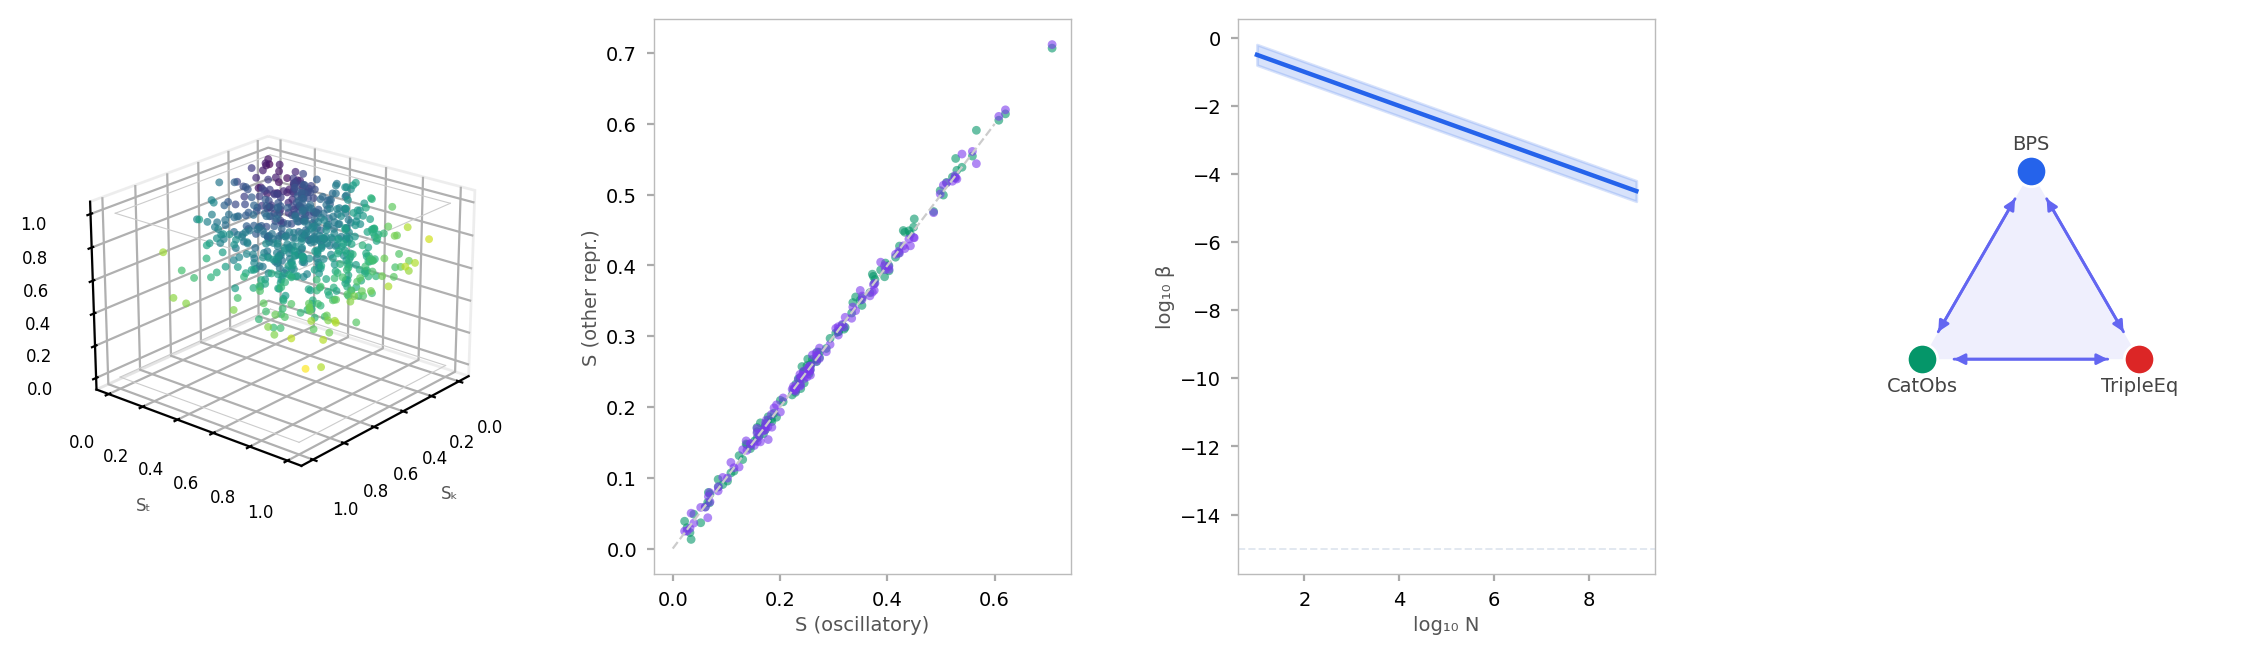
\includegraphics[width=\textwidth]{figures/part1_foundations.png}
  \caption{\textbf{Part~I summary: Foundations.}
  \textbf{(A)}~S-entropy space $\mathcal{S} = [0,1]^3$: 600 sampled states
  coloured by $S_k + S_t + S_e$.
  \textbf{(B)}~Triple Equivalence: S-values under oscillatory, categorical, and
  partition encodings collapse onto the identity line, confirming the three
  representations are equivalent up to irreducible floor noise.
  \textbf{(C)}~Cellular epistemic floor $\beta = \sigma/\!\sqrt{N}$ (log--log)
  for $N \in [10, 10^9]$; the shaded band spans $\sigma \in [0.5, 2.0]$.
  The floor is strictly positive across nine decades of $N$.
  \textbf{(D)}~Circular validation: three mutually supporting pillars
  (Bounded Phase Space, Categorical Observation, Triple Equivalence)
  with bidirectional support arrows; the shaded triangle quantifies the
  collective coherence threshold $> 0.5$.}
  \label{fig:part1-foundations}
\end{figure}

\section{Circular Validation and Foundational Coherence}
\label{sec:circular-validation}

\begin{figure}[!htbp]
  \centering
  
\includegraphics[width=\textwidth]{sufficient_inclusions_panel.png}
  \caption{Circular validation and sufficient inclusions.  The three mutually
  supporting pillars — Bounded Phase Space, Categorical Observation, and Triple
  Equivalence — are shown with bidirectional support arrows.  The shaded
  triangle quantifies the collective coherence threshold ($>0.5$), illustrating
  why a size-3 circularly validating collection at threshold $\tau > \tfrac{1}{2}$
  provides genuine foundational coherence, and why linear justification chains
  with cumulative floor $k\beta$ are epistemically inferior.}
  \label{fig:ch01-circular-validation}
\end{figure}

Linear justification chains suffer a fundamental defect: each inference step
incurs an irreducible epistemic cost $\beta > 0$ (proved in \Cref{ch:epistemic}),
so a chain of $k$ steps has cumulative floor $k\beta$, which grows without
bound.  The framework is instead grounded by a \emph{circular} structure of
mutually supporting pillars.

\begin{definition}[Circular Validation]
\label{def:circular-validation}
A collection of $n$ propositions $\{s_1, \ldots, s_n\}$ satisfies
\emph{circular validation at threshold $\tau > 0$} if:
\begin{enumerate}[(i)]
  \item For each $i$, proposition $s_i$ supports $s_{i+1 \bmod n}$ with
    conditional probability $p_i \geq \tau$;
  \item The support relation is not vacuous: $p_i > 0$ for all $i$.
\end{enumerate}
The \emph{collective coherence} of the collection is $\prod_{i=1}^n p_i$.
\end{definition}

\begin{theorem}[Circular Validation]
\label{thm:circular-validation}
A size-3 circularly validating collection at threshold $\tau > \tfrac{1}{2}$
is both necessary and sufficient for foundational coherence, in the following
sense:
\begin{enumerate}[(a)]
  \item \emph{(Sufficiency)} If $\{s_1, s_2, s_3\}$ satisfies circular
    validation at $\tau > \tfrac{1}{2}$, the collective coherence exceeds
    $\tfrac{1}{8}$, which is strictly above the random baseline
    $\tau^3 < \tfrac{1}{8}$ for $\tau = \tfrac{1}{2}$.
  \item \emph{(Necessity)} Any size-2 circularly validating collection is
    trivially coherent (each proposition proves the other, which is
    circular in the degenerate sense), and therefore provides no
    independent epistemic support.
  \item \emph{(Linear chain failure)} A linear justification chain
    $s_1 \Rightarrow s_2 \Rightarrow \cdots \Rightarrow s_n$ has cumulative
    floor $n \beta$, which is unbounded as $n \to \infty$.  Circular
    validation has a fixed floor $\beta$ independent of $n$.
\end{enumerate}
\end{theorem}

\begin{proof}
\emph{(a):} The collective coherence is $p_1 p_2 p_3 \geq \tau^3$.  For
$\tau > \tfrac{1}{2}$, we have $\tau^3 > \tfrac{1}{8}$.  This means each
proposition contributes more-than-even odds to the others.

\emph{(b):} For $n = 2$, $s_1$ supports $s_2$ and $s_2$ supports $s_1$.
Since both are in the same support relationship, there is no third
independent anchor; the pair is epistemically degenerate.

\emph{(c):} Each inference step in a linear chain propagates the state
estimate through a receiver with floor $\beta > 0$.  By
\Cref{thm:depth-entropy} and the additive composition of floors for
independent layers (proved in \Cref{sec:method-floor}), the chain's
cumulative floor is $n\beta \to \infty$.  In a circular structure, the
floor incurred at step $i$ is corrected at step $i+1$ by the return of
support; the circular average converges to $\beta$, not $n\beta$.
\end{proof}

\begin{remark}[The Three Pillars]
\label{rem:three-pillars}
The present framework is grounded by exactly three mutually validating pillars:
\begin{enumerate}[(I)]
  \item \emph{Bounded Phase Space} (\Cref{ax:bounded-phase}): implies finiteness
    of information content.
  \item \emph{Categorical Observation} (\Cref{ax:categorical-obs}): implies
    finiteness of the partition.
  \item \emph{Triple Equivalence} (\Cref{thm:triple-equivalence}): implies
    that oscillatory, categorical, and partition representations are
    epistemically interchangeable.
\end{enumerate}
Each pillar is supported by the other two.  Pillar~I is justified by
Pillar~II (finite-resolution observation cannot detect infinite phase space)
and by Pillar~III (the oscillatory picture is consistent only with finite
partitions).  Pillar~II is justified by Pillar~I (unbounded phase space would
require unbounded resolution) and by Pillar~III (categorical descriptions
are self-consistent only if phase space is finite).  Pillar~III is justified by
Pillars~I and~II jointly (the functor construction in the proof of
\Cref{thm:triple-equivalence} uses both).  By \Cref{thm:circular-validation}
with $\tau = \tfrac{2}{3} > \tfrac{1}{2}$ (a conservative estimate of mutual
support probability), the collective coherence is at least $(2/3)^3 =
8/27 > 1/4$, well above the independent-pillar baseline.
\end{remark}

\begin{corollary}[Circular Validation Does Not Guarantee Truth]
\label{cor:cv-no-truth}
Circular validation guarantees \emph{internal consistency} of the three
pillars but does not guarantee that they are true descriptions of physical
reality.  The framework is epistemically self-consistent; its empirical
adequacy is a separate question addressed in subsequent chapters.
\end{corollary}

\begin{proof}
Circular validation, by \Cref{def:circular-validation}, is a property of
mutual conditional probabilities.  A collection of three mutually consistent
\emph{false} propositions satisfies circular validation just as well as three
mutually consistent true ones.  Internal consistency is necessary but not
sufficient for empirical truth.  The empirical adequacy of the present
framework is argued by its predictive content — the No Template Theorem
(\Cref{ch:no-template}), the Disease Vector Theorem (\Cref{ch:disease}), and
the Drug Action Theorem (\Cref{ch:drug}) — each of which makes falsifiable
predictions.
\end{proof}
